\chapter{Implementation} \label{implementation}


\section{Overview}

This chapter details the implementation of a robotic mapping and image processing pipeline designed for spatial mapping with a Turtlebot4 robot. Leveraging the capabilities of the Spectacular AI SDK and ROS2, I developed a custom ROS2 node that performs real-time mapping on the Turtlebot4. This node captures environmental data and processes it to generate keyframe-based mapping suitable for autonomous navigation and further spatial analysis.

In addition to the mapping node, I implemented secondary ROS2 nodes running on a laptop, responsible for saving images, their poses and the calculated pointcloud captured at keyframe intervals. This process allows for high-resolution image and pose acquisition, preserving critical visual information for later post-processing. A post-process script subsequently cleans the image set by discarding blurry or overexposed images. This refined set of images, the poses and the pointlcoud is then used as input to Gaussian Splatting.

To enhance the 3D model, I applied Gaussian splatting to generate a smooth, visually coherent representation of the mapped environment. This pipeline supports high-quality spatial mapping with applications in various robotic and industrial domains, providing accurate visual models essential for analysis and further computational tasks.

\section{Mapping}

After our experiments with RTAB-Map and nvblox (see Chapter~\ref{experiments_3d_mapping}) it became clear that they are not suitable for our expectations. Due to RTAB-Map's lag and frequent lose of track and NVIDIA Isaac VSLAM's (and nvblox's) hardware requirements we did not want to use them in the implementation of the mapping. On the other hand, the Spectacular AI SDK proved itself to be precise in our experiments (see Section~\ref{experiments_spai}) and we did not have to invest in additional hardware, so we decided to proceed with it in the implementation. 

I created a ROS2 workspace for the robot which has a package that contains my \verb|spectacularai_node|. The node is the core component of our mapping implementation and is responsible for generating and publishing spatial data essential for real-time SLAM (Simultaneous Localization and Mapping). The node, located within the \verb|spectacularai_depthai_turtlebot| package, is built with the Spectacular AI SDK, which offers precise Visual-Inertial Odometry (VIO) and SLAM capabilities optimized for robotic applications.

The node initializes several ROS2 publishers that communicate mapping and image data. Key topics include \verb|/slam/odometry| for publishing the estimated pose, \verb|/tf| for broadcasting the transformation tree, \verb|/slam/left| for transmitting image data from the left camera, \verb|/slam/keyframe| for transmitting keyframe poses, \verb|/slam/pointcloud| for 3D point cloud data, and \verb|/slam/camera_info| to share camera intrinsic information.

Key methods in \verb|spectacularai_node| are as follows:
\begin{itemize}
    \item \verb|processOutput|: Monitors the VIO session output and processes each available frame.
    \item \verb|onVioOutput|: Called for each VIO output, publishing the odometry and TF data based on the calculated pose, which includes both position and orientation in the world frame.
    \item \verb|onMappingOutput|: This callback handles mapping outputs, iterating through updated keyframes and invoking methods to store and publish them.
    \item \verb|newKeyFrame|: Extracts pose and image data from keyframes, publishing each frame as a ROS2 message. The keyframe pose is converted to \textit{PoseStamped} format, while left-camera images are published via the \textit{CvBridge}.
    \item \verb|publishPointCloud|: Computes a 3D point cloud using position data transformed by the camera’s pose matrix. This point cloud is then published as a \textit{PointCloud2} message.
\end{itemize}

After launching the node on the robot we got an error that the Spectacular AI Python SDK is not installed. We were not able to install it because, unless on \textit{x86} CPU architecture it is free, users have to pay for it to use on the \textit{aarch64} architecture (the robot's controller is a Raspberry Pi 4). After consulting with my advisor he suggested that I should ask the Spectacular AI Team if they would grant me the SDK for my thesis. I submitted a form on their website with my university e-mail address provided as my contact address and after a week they provided me the \textit{.whl} files of the Python SDK. I want to thank and give my best regards to the Spectacular AI Team and Jerry Ylilammi who gave me access to these files. With the Python SDK installed we were finally able to start the node successfully.

In addition to the robot’s workspace, a secondary ROS2 workspace was created specifically for a notebook situated on the Turtlebot4’s platform. This workspace comprises 4 packages: \verb|rviz2_laptop|, \verb|keyframe_saver|, \verb|pointcloud_saver| and \verb|camera_info_saver|. The \verb|rviz2_laptop| package contains a launch file to initiate RViz, allowing for real-time visualization of data generated by the \verb|spectacularai_node|. This capability facilitates interactive monitoring and helps verify the mapping accuracy while the robot is in operation. The RViz visualized mapping of my mapping node can be seen on Figure~\ref{fig:spai_mapping_rviz}

\begin{figure}[htbp]
	\centering
	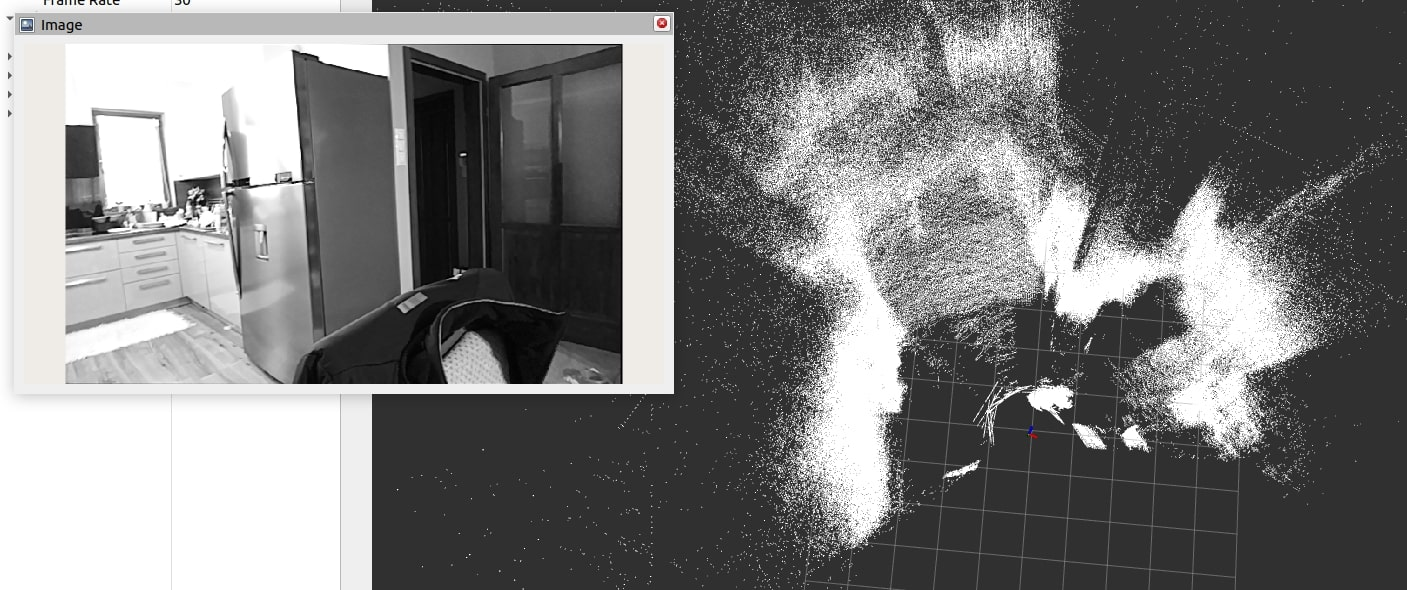
\includegraphics[width=150mm, keepaspectratio]{figures_jpg/spai_mapping_rviz.jpg}
	\caption{Mapping with Spectacular AI, visualized by RViz, point cloud from above}
	\label{fig:spai_mapping_rviz}
\end{figure}


\section{Saving and processing data for Gaussian splatting}

The \verb|CameraInfoSaver| node in the \verb|camera_info_saver| package is a ROS2 utility designed to extract and store camera intrinsic parameters from \verb|CameraInfo| messages published on the \verb|/slam/camera_info| topic. This node plays a critical role in generating datasets for 3D reconstruction and SLAM applications by capturing essential camera calibration data required for accurate pose estimation and scene modeling in Gaussian Splatting. This node extracts the image dimensions (height and width) and the intrinsic matrix (\textbf{K}), including focal lengths (fl\_x, fl\_y) and principal points (cx, cy). The node captures the distortion model and the complete intrinsic matrix as well. The extracted data is saved as a JSON file, ensuring compatibility with downstream processes that require camera calibration parameters.

The package called \verb|keyframe_saver|, implements a ROS2 node that subscribes to two topics: \verb|/slam/left| and \verb|/slam/keyframe|. This node, titled \textit{KeyframeImageSaver}, is responsible for capturing and saving images and poses whenever a keyframe pose is detected. The node’s code leverages OpenCV, alongside ROS2's \verb|cv_bridge|, to convert incoming ROS \textit{Image} messages to OpenCV-compatible images. When a new keyframe pose is received on the \verb|/slam/keyframe| topic, the node retrieves the latest image from \verb|/slam/left|, converts it, and stores it in a designated directory with a sequential filename. When a keyframe message is received the node saves the latest pose into a \verb|json| file into the same folder as the images, named sequentially.

The \verb|PointCloudSaver| node is another ROS2 component of my pipeline designed to capture and save 3D point cloud data from the \verb|/slam/pointcloud| topic. It ubscribes to the \verb|/slam/pointcloud| topic to receive \verb|PointCloud2| messages containing 3D spatial data and, in addition, to the \verb|/slam/keyframe| topic to trigger saving the most recent point cloud when a keyframe pose is published. The point cloud data is saved in the PLY (Polygon File Format) file format~\cite{ply_format}, widely used for storing 3D models and point cloud data. The file is initialized with a header specifying the ASCII format, vertex structure, and placeholder for the vertex count. Subsequent point data is appended to the file. The header's element vertex count is dynamically updated after each save operation to ensure file consistency.

These functionality are essential to the mapping workflow, as the saved data serve as the basis for further processing. There are 2 main post-processing scripts that prepare the collected dataset for photorealistic reconstruction:
\begin{itemize}
    \item one for image processing,
    \item the other one for pose and point transformation and dataset copying.
\end{itemize}

\subsection{Image processing}

The image post-processing script used in this thesis further refines the keyframe images captured by the \textit{KeyframeImageSaver} node. By automatically identifying and discarding low-quality images — namely, those that are either blurry or overexposed — this script ensures that only high-quality images are retained for the photogrammetry reconstruction process. After filtering, the script renames the remaining images in a sequential order, which aids in organizing the dataset for subsequent processing steps.

To determine if an image is blurry, the script employs the variance of the Laplacian method~\cite{blur_detection}. This method calculates the variance of pixel intensity in the Laplacian of the grayscale version of the image. The Laplacian operator is defined as the sum of second-order partial derivatives:

\begin{equation}
 \triangle \mathit{f}\left (x,y  \right )= \frac{\partial^2 f }{\partial x^2} + \frac{\partial^2 f }{\partial y^2}
\end{equation}

where \(f(x,y)\) represents the grayscale image intensity at pixel location \((x,y)\). Variance measures the spread of values around the mean; a high variance indicates sharpness (high contrast edges), while a low variance suggests blurriness (low contrast edges). In this script, we define a threshold for variance: if the computed variance is below this threshold, the image is considered blurry and is flagged for deletion. 
The corresponding code snippet can be inspected here:

\FloatBarrier
\begin{lstlisting}[language=python,frame=single,float=!ht]
def is_blurry(image_path, threshold):
    """Check if an image is blurry using the variance of the Laplacian."""
    image = cv2.imread(image_path, cv2.IMREAD_GRAYSCALE)
    if image is None:
        return False
    laplacian_var = cv2.Laplacian(image, cv2.CV_64F).var()
    return laplacian_var < threshold
\end{lstlisting}
\FloatBarrier

In this function, \verb|cv2.Laplacian| calculates the Laplacian of the grayscale image, and \verb|.var()| computes the variance of the resulting matrix. If \verb|laplacian_var| is less than the threshold, the image is deemed blurry. I adjusted the threshold by doing experiments with blurry images, it performed best with the value of 500.

For overexposure detection, the script evaluates the average brightness of an image. An overexposed image typically has a high overall intensity across the majority of pixels, indicating that many parts of the image are too bright. This approach converts the image to grayscale and calculates the mean pixel value. If the mean brightness exceeds a predefined threshold, the image is considered overexposed.

The mathematical foundation here is based on calculating the mean of pixel intensities (\(I\)) in a grayscale image, which is computed as:
\begin{equation}
    \textbf{Mean Brightness} = \frac{1}{N}\sum_{i=1}^{N} I\left ( i \right )
\end{equation}
where \(N\) is the total number of pixels in the image. A high mean value signifies overexposure.

The code for overexposure detection is as follows:

\FloatBarrier
\begin{lstlisting}[language=python,frame=single,float=!ht]
def is_overexposed(image_path, brightness_threshold):
    """Check if an image is overexposed based on brightness levels."""
    image = cv2.imread(image_path)
    if image is None:
        return False
    gray = cv2.cvtColor(image, cv2.COLOR_BGR2GRAY)
    mean_brightness = np.mean(gray)
    return mean_brightness > brightness_threshold
\end{lstlisting}
\FloatBarrier
Here, \verb|np.mean(gray)| computes the average brightness, and if this value exceeds the \verb|brightness_threshold|, the image is flagged for deletion. I adjusted the threshold by doing experiments with overexposed images, it performed best with the value of 200.

After the detection of overexposed and blurry images the script iterates over all images in the specified directory, deletes any images identified as blurry or overexposed, and finally renames the remaining images in a sequential order. This ensures a clean, orderly dataset that is ready for the reconstruction pipeline.

By filtering out suboptimal images, this script plays a crucial role in optimizing the dataset, ensuring that the photogrammetry process has a higher chance of generating accurate 3D reconstructions. This refinement contributes to the overall quality and reliability of the map generated in the final stages of processing.

\subsection{Pose and point transformation}

The pose and point transformation script plays a vital role in converting data collected from the ROS2 pipeline into the format required by SplatFacto in NeRFStudio. This script processes the positional and orientational data, performs necessary coordinate transformations, and organizes the dataset structure.

The transformations are applied to align the data with the conventions used in NeRFStudio, which follows the OpenGL/Blender coordinate system~\cite{opengl_coordinate_system}, where \(+X\) is right, \(+Y\) is up and \(-Z\) is the look-at direction. To achieve this, two main transformation matrices are used:

\begin{itemize}
    \item Robotics to vision transformation matrix
    \item Vision to graphics transformation matrix
\end{itemize}

They are defined as follows:
\[
T_\text{vision\_to\_graphics} = \begin{bmatrix}
1 & 0 & 0 & 0 \\
0 & -1 & 0 & 0 \\
0 & 0 & -1 & 0 \\
0 & 0 & 0 & 1
\end{bmatrix}
\]

\[
T_\text{robotics\_to\_vision} = \begin{bmatrix}
0 & -1 & 0 & 0 \\
0 & 0 & -1 & 0 \\
1 & 0 & 0 & 0 \\
0 & 0 & 0 & 1
\end{bmatrix}
\]

The script processes positional and orientational data provided as json files for each keyframe. These values are converted into \(4\times4\) transformation matrices that align the data with the NeRFStudio graphics coordinate system.

The pipeline involves the following steps:
\begin{enumerate}
    \item Loading Camera Intrinsics: The script reads intrinsic parameters from \verb|camera_info.json|, including focal lengths, principal points, and image dimensions, ensuring compatibility with NeRFStudio's input format.
    \item Folder Structure Creation: It creates the required folder structure and copies images and poses into designated directories.
    \item Pose and point Conversion: Using the transformation matrices, the poses and pointcloud in robotics conventions are converted to NeRFStudio graphics conventions. This ensures correct alignment of the 3D models with the dataset.
    \item Dataset Creation: A \verb|transforms.json| file is generated, combining the transformed poses, intrinsic parameters, and file paths. This file includes:
    \begin{itemize}
        \item File paths to images.
        \item 4×4 transformation matrices for each keyframe.
        \item Intrinsic parameters.
        \item Reference to the transformed point cloud file.
    \end{itemize}
\end{enumerate}

The key function for pose conversion is outlined below:
\FloatBarrier \begin{lstlisting}[language=python,frame=single,float=!ht]
def pose_to_transform_matrix(position, orientation):
    """Convert position and orientation to a 4x4 transformation matrix."""
    translation = np.array([position["x"], position["y"], position["z"]])
    rotation = R.from_quat([orientation["x"], orientation["y"], orientation["z"], orientation["w"]])
    
    # Initial transformation matrix
    pose_robotics = np.eye(4)
    pose_robotics[:3, :3] = rotation.as_matrix()
    pose_robotics[:3, 3] = translation

    # Transforming the matrix
    pose_vision = T_vision_to_robotics @ pose_robotics
    pose_graphics = pose_vision @ T_vision_to_graphics

    return pose_graphics.tolist()
\end{lstlisting}

The script also transforms the points (vertexes) in the pointcloud into the required coordinate system:
\FloatBarrier \begin{lstlisting} [language=python,frame=single,float=!ht]
for idx, line in enumerate(vertex_data):
    x, y, z = map(float, line)
    vertex_coords = np.array([x, y, z, 1])
    transformed_point = T_vision_to_robotics @ vertex_coords
    f.write(f"{transformed_point[0]} {transformed_point[1]} {transformed_point[2]}\n")
\end{lstlisting}

\subsection{Gaussian splatting}

With the filtered images, the camera intrinsics and the transformed poses and pointclouds we are ready for creating the Gaussian splat. The next is step is to train the Gaussian splat model using the \verb|ns-train| command. The usage can be seen here:
\FloatBarrier
\begin{lstlisting}[language=bash,frame=single,float=!ht]
ns-train splatfacto --data gsplat_input/
\end{lstlisting}
\FloatBarrier

The command initiates the training of the Gaussian splat model on the processed data in the \verb|gsplat_input/| folder. After the training has started the process can be inspected via the viewer as seen on Figure~\ref{fig:training_nerf_karcag}.

This step is a core component of the pipeline, wherein the neural model learns to reconstruct scenes using Gaussian splatting. The model leverages the processed images to produce a probabilistic representation of the 3D environment, ideal for generating photorealistic splats.

When the training is complete, a created splat can be exported into a \verb|.ply| file with the following command:
\FloatBarrier
\begin{lstlisting}[language=bash,frame=single,float=!ht]
ns-export gaussian-splat --load-config outputs/gsplat_input/splatfacto/DATE/config.yml --output-dir exports/splat/\end{lstlisting}
\FloatBarrier
The saved file then can be opened with a Gaussian splat viewer and the created splat can be inspected.

\section{Laci: Gabor, where should I put the link to my repository?}
